\documentclass[border=4pt,tikz]{standalone}
\usepackage[utf8]{inputenc}
\usepackage[T1]{fontenc}
\usepackage{tikz}
\usepackage{xcolor}
\usetikzlibrary{positioning, shapes.geometric, arrows.meta, calc}
\definecolor{nodeFill}{HTML}{E8EEF7}
\definecolor{nodeStroke}{HTML}{1F3A5F}
\definecolor{accent}{HTML}{3D5A80}
\definecolor{soft}{HTML}{F4F1EA}
\definecolor{softStroke}{HTML}{8B7355}
\definecolor{decision}{HTML}{FFF4E0}
\definecolor{decisionStroke}{HTML}{B8860B}
\definecolor{textDark}{HTML}{1A1A1A}
\begin{document}
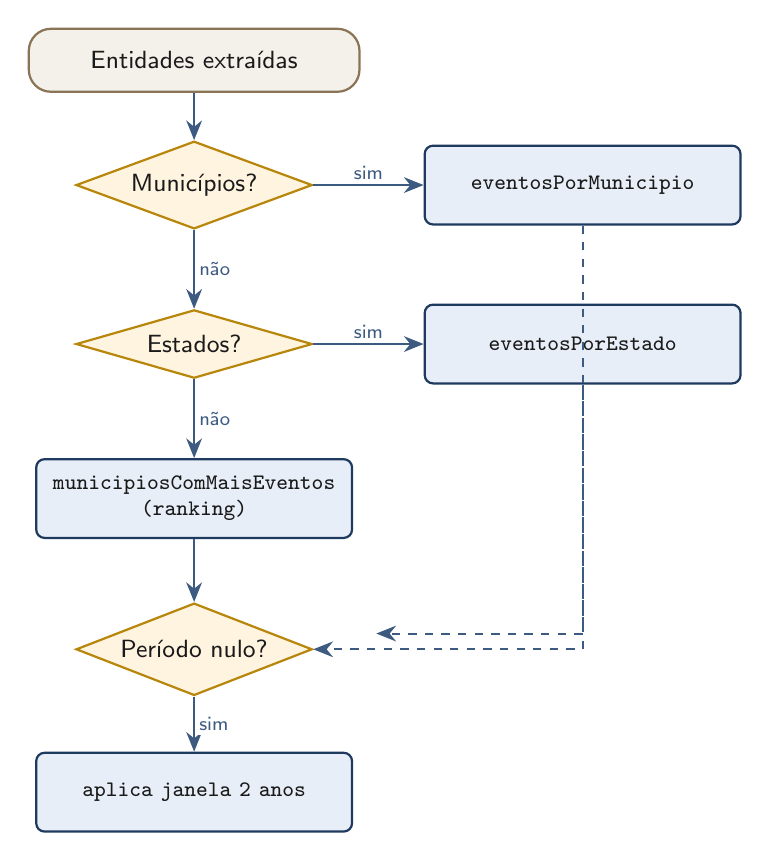
\begin{tikzpicture}[
  font=\sffamily\small,
  every node/.style={text=textDark},
  start/.style={
    rectangle, rounded corners=8pt,
    draw=softStroke, line width=0.8pt, fill=soft,
    minimum width=42mm, minimum height=8mm,
    align=center
  },
  decision/.style={
    diamond, aspect=2.2,
    draw=decisionStroke, line width=0.8pt, fill=decision,
    minimum width=30mm, inner sep=1pt, align=center
  },
  action/.style={
    rectangle, rounded corners=3pt,
    draw=nodeStroke, line width=0.8pt, fill=nodeFill,
    text width=38mm, minimum height=10mm, align=center,
    font=\sffamily\footnotesize\ttfamily, inner sep=3pt
  },
  flow/.style={
    -{Stealth[length=2.5mm, width=2mm]},
    draw=accent, line width=0.7pt
  },
  edgelabel/.style={
    font=\sffamily\scriptsize, text=accent,
    fill=white, inner sep=1.5pt
  }
]
  \node[start] (start) {Entidades extraídas};
  \node[decision, below=6mm of start] (d1) {Municípios?};
  \node[action, right=14mm of d1] (a1) {eventosPorMunicipio};
  \node[decision, below=10mm of d1] (d2) {Estados?};
  \node[action, right=14mm of d2] (a2) {eventosPorEstado};
  \node[action, below=10mm of d2] (a3) {municipiosComMaisEventos\\(ranking)};
  \node[decision, below=8mm of a3] (d3) {Período nulo?};
  \node[action, below=7mm of d3] (a4) {aplica janela 2 anos};

  \draw[flow] (start) -- (d1);
  \draw[flow] (d1.east) -- (a1.west) node[edgelabel, midway, above] {sim};
  \draw[flow] (d1.south) -- (d2.north) node[edgelabel, midway, right] {não};
  \draw[flow] (d2.east) -- (a2.west) node[edgelabel, midway, above] {sim};
  \draw[flow] (d2.south) -- (a3.north) node[edgelabel, midway, right] {não};
  \draw[flow] (a3.south) -- (d3.north);
  \draw[flow, dashed] (a1.south) |- ($(d3.east) + (10mm,0)$) -- (d3.east);
  \draw[flow, dashed] (a2.south) |- ($(d3.east) + (8mm,2mm)$);
  \draw[flow] (d3.south) -- (a4.north) node[edgelabel, midway, right] {sim};
\end{tikzpicture}
\end{document}
